\chapter{Flutter Foundations}
\label{ch:flutter}
In the introduction, a new, promising, cross-platform framework was introduced. The Flutter's primary goal is to provide the ability to build high-performance, high-fidelity apps for \textit{iOS}, \textit{Android}, web, and desktop systems (Windows, MacOS) from a single code-base~\cite{flutter-technical-overview}. In this chapter, the~framework philosophy will be described. Used programming language and theory of reactive programming is briefly introduced. The chapter describes the concept of widgets as a base building block for every application. Later on, one of the most critical topics -- \textit{state management} is discussed in the~form of existing approaches and recommendation which to prefer when building applications. At the end of this chapter, the brief look under the framework's hood is discussed.

Flutter includes a modern react-style framework, a 2D rendering engine, predefined widgets and development tools. The primary premise is a motto ``everything is a widget''. A widget is an immutable building block of application which is part of the user interface. Each widget can define structural elements such as a~button, stylistic elements such as colour or it can define the interface's layout, such as padding. Widgets are composed as a tree hierarchy with a~possibility of composing each widget to another. If any event occurs (such as user interaction), the framework can rebuild part of this tree to redraw the screen.  

\begin{figure}[htp]
    \centering
    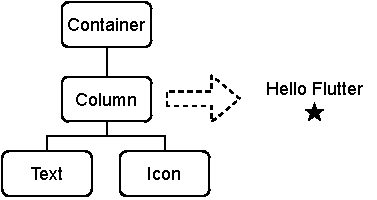
\includegraphics[width=0.5\linewidth]{img/flutter/hello-flutter.pdf}
    \caption{Widget composition example}
    \label{fig:hello-flutter}
\end{figure}

Flutter encourages developers to create and use small, single-purpose widgets and compose them to create complex interfaces and layouts. Take an~example from~\Cref{listing:hello-flutter}, where the root widget, Container, is used to create a rectangular visual element. The Container is something like <div> element in HTML. Under the Container there is Column widget which composes children widgets into the vertical direction. Finally, Text widget displaying text ``Hello Flutter'' and Icon widget showing star icon. The~composition hierarchy along with a~result is shown in~\Cref{fig:hello-flutter}.

\begin{listing}[ht]
\begin{minted}{dart}
Container(
    padding: const EdgeInsets.all(5.0),
    child: Column(
      mainAxisAlignment: MainAxisAlignment.center,
      children: [
        Text('Hello Flutter'),
        Icon(Icons.star),
      ]
    ),
)
\end{minted}
\caption{Widget composition code example}
\label{listing:hello-flutter}
\end{listing}
% ----- % ----- % ----- % ----- % ----- % ----- % ----- % ----- % ----- % ----- % ----- % ----- % ----- % ----- %
\section{Technical overview}
Flutter uses programming language \textit{Dart}~(specification v2.0~\cite{dart-specs}). It is also made by Google and it is inspired by languages such as JavaScript. Dart using statically typed system with runtime checks, but like many other languages highly use type inference~\cite{dart-type-system}. Dart can be used from writing simple scripts to full-featured applications. Dart has flexible compiler technology where the compiler can decide running code in different ways, depending on the targeted platform~\cite{dart-platforms}. 

\begin{itemize}
    \item \textbf{Dart Native} -- For programs targeting devices (mobile, desktop, server, and more), Dart Native includes both a Dart VM with \gls{jit} compilation and an~\gls{aot} compiler for producing machine code.
    \item \textbf{Dart Web} -- For programs targeting the web, Dart Web includes both a development time compiler (dartdevc) and a production time compiler (dart2js).
\end{itemize}

\begin{figure}[htp]
    \centering
    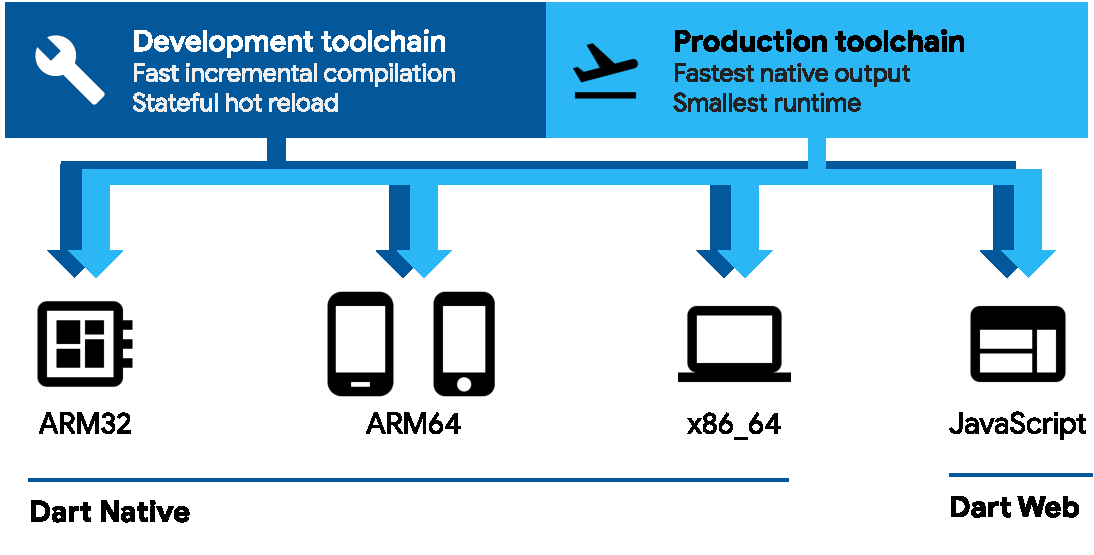
\includegraphics[width=0.8\linewidth]{img/flutter/dart-platforms.pdf}
    \caption{Dart platforms~\cite{dart-platforms}}
    \label{fig:dart-platform}
\end{figure}

Flutter performs the use of both ways. If the targeted platform is web, the \textit{Dart~Web} is used. For other platforms \textit{Dart~Native} is chosen. The Dart~Native's \gls{jit} compilation is highly used to support fast development process with ``hot-reload'' functionality. Then the~\gls{aot} compilation is used for the best-optimised production-ready result on the native platform.  

Flutter framework is organised into several layers (see~\Cref{fig:flutter-layer-cake}), where each layer makes usage of the previous one. The upper layers are more frequently used by developers on a daily basis, and lower layers are used only if the developers need to create particular customizations. 

\begin{figure}[htp]
    \centering
    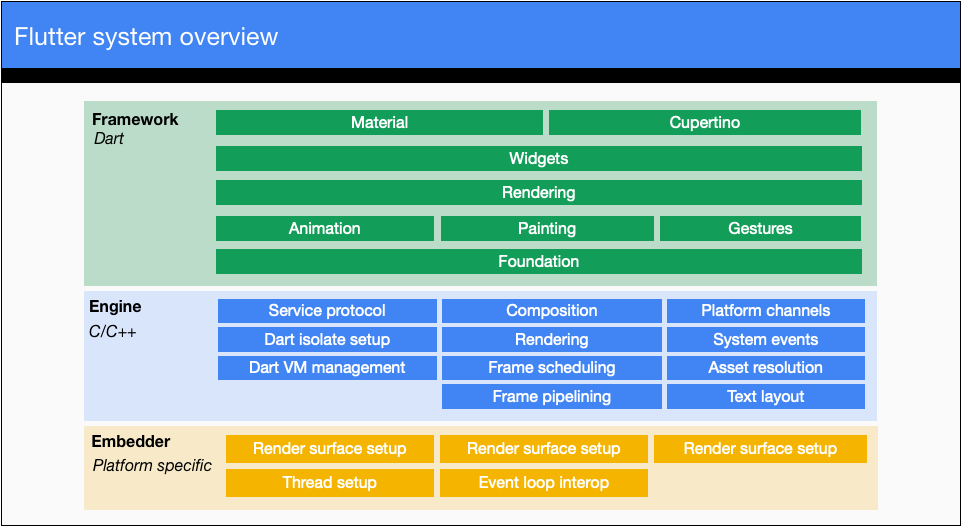
\includegraphics[width=0.8\linewidth]{img/flutter/flutter-layer-cake.png}
    \caption{Flutter system overview~\cite{flutter-technical-overview}}
    \label{fig:flutter-layer-cake}
\end{figure}

Unlike the other frameworks, Flutter uses high-performance 2D rendering engine and draws everything onto the~screen directly. That means pixel-perfect control over what and how it is displayed. The most top layers, \textit{Material} and \textit{Cupertino}, are set of widgets which defines Material Design (Android systems) and Apple Design components respectively. To highlight that, Flutter does not use native components, but everything draws by itself. These two layers support developers to bring the standardised look and feel to the targeted platform.
% --- # --- # --- # --- # --- # --- # --- # --- # --- # --- # --- # --- # --- # --- # --- # --- # --- # --- #
\subsection{Reactive Programming}
Flutter makes significant usage from the concept of reactive programming. There is nearly always a~requirement to update data in response to user interaction or any other event such as getting data from the~server. More than that, sometimes it is necessary to update different parts of the user interface in response to these events. 

Flutter creates user interface by composing \textbf{immutable} widgets. The immutability is the key point here. Whenever user interface needs to ``redraw'' screen, the~part of the~widget tree is replaced by \textbf{new} widget instances (in fact, it is not simple as that, and this topic is more deeply discussed later in this chapter). In many other \gls{ui} frameworks, such as \textit{Xamarin}, is usually taken the approach of coupling \gls{ui} components with view-models through concepts such as data binding~\cite{xamarin-data-binding}. That means that whenever \gls{ui} needs to~change, the~components mutate application's state. Flutter takes an~entirely different approach. It can be said ``here is the current state of the application, draw something on the screen accordingly''.

\subsubsection{The Notion of Streams}
A Stream can be described as ``a pipe with two ends, only one allowing to insert something into it. When something is inserted into the pipe, it flows inside the pipe and goes out by the other end''~\cite{reactive-didier}. The~Stream can convey any~data type, from simple values to~events, complex object or even another stream. The~data can come to the~Stream, for example, from an external data source such as server connection or from events such as user interactions. In Dart, the Streams support manipulating them, filtering, re-grouping, modify data before they are send and much more. This functionality can be used to build reactive \gls{ui}. Flutter has several widgets supporting streams to rebuild part of the~\gls{ui} whenever new data arrived into the~Stream.

The answer to the question ``What is reactive programming?`` could be ``Reactive programming is programming with asynchronous data streams``~\cite{reactive-didier}\cite{reactive-red-hat}. Within Flutter framework, anything from an interaction event (tap, gesture), changes of a variable, messages, everything that may change is conveyed and triggered by streams.

It means that with reactive programming, according to~\cite{reactive-didier}, the~application:

\begin{quote}
    \begin{itemize}
        \item becomes asynchronous,
        \item is architectured around the notion of Streams and their listeners,
        \item when something happens somewhere (an event, a change of a variable) a~notification is sent to a~Stream,
        \item if ``somebody'' listens to that Stream, it will be notified and will take appropriate action(s), whatever its location in the~application.
    \end{itemize}
    
    From Widgets perspective -- Widget does not longer need to know:
    
    \begin{itemize}
        \item what is going to happen next,
        \item who might use this information (no one, one or several Widgets),
        \item where this information might be used (nowhere, same screen, another one, several ones),
        \item when this information might be used (almost directly, after several seconds, never).
    \end{itemize}
\end{quote}

Later on in this chapter, the pattern Business Logic Component (BLoC) is introduced. This pattern uses Streams to manage application life-cycle and are used for state management.
% ----- % ----- % ----- % ----- % ----- % ----- % ----- % ----- % ----- % ----- % ----- % ----- % ----- % ----- %
\section{Everything Is a Widget}
In this section, we will discuss in more detail how the~\gls{ui} is built. Every \gls{ui} consists of the layout and individual components. The layout defines the screen's base structure, such as a menu on the top and subsequent actions on the bottom. Then the layout is composed of individual components, such as a menu, buttons or icons. Together they create a final interface.

These building blocks in Flutter are called ``Widgets''. Whatever it is simple text, a button, or complex parts of the~layout, such as a~grid with multiple columns and rows -- \textbf{everything is a widget}.  Widgets describe what their view should look like given their current configuration and state. When a widget's state changes, the widget rebuilds its description, which the framework diffs against the previous description in order to determine the minimal changes needed in the underlying render tree to transition from one state to the next one~\cite{flutter-widget-intro}. As the~composition to the~tree implies, each widget has at most one parent and zero or more children widgets. This tree, called ``widget tree'', is in fact, one of the~three trees involved. The~framework has a sophisticated way of decision about how the~trees should be rebuilt and the~screen updated. This behaviour is in more detail described later in this chapter.

The Flutter framework uses only one language to define both the~user interface and business logic as well.  Widgets are Dart class which inherits from some of the widget's base class (typically \textit{StatelessWidget} or \textit{StatefulWidget}). Each widget has a build method which defines how the widget should be built (and drawn on the screen). 
% --- # --- # --- # --- # --- # --- # --- # --- # --- # --- # --- # --- # --- # --- # --- # --- # --- # --- #
\subsection{Widgets Are Not Only Visible Parts}
Widgets are not only visible parts of the \gls{ui} such as clickable buttons, text or icons. The widgets also define layouts such as columns, rows, grids, the margin between other widgets, padding around them and more. 

\begin{figure}[htp]
    \centering
    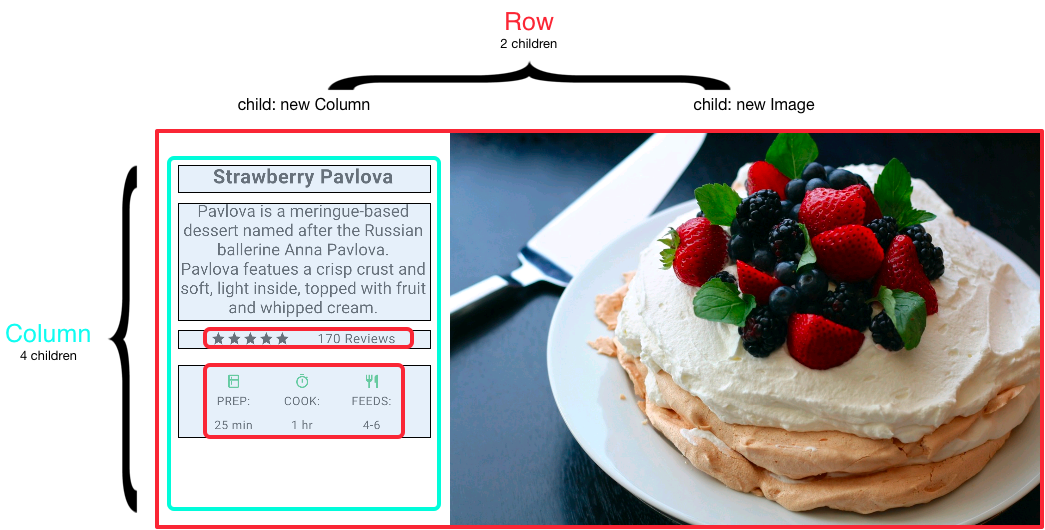
\includegraphics[width=0.9\linewidth]{img/flutter/layout_compose.png}
    \caption{Compose widgets to create layout~\cite{flutter-widget-layout}}
    \label{fig:flutter-compose-widget}
\end{figure}

An example of widget composition creating a~layout is shown in~\Cref{fig:flutter-compose-widget}. The root widget, a~\textit{Row} widget, contains two nested widgets. On the~left there is a~\textit{Column} which contains more nested widgets and on the~right, \textit{Image} widget which displays a~product image. The~break-down of the left column widget can be seen in~\Cref{fig:flutter-compose-widget-detail}. 

\begin{figure}[htp]
    \centering
    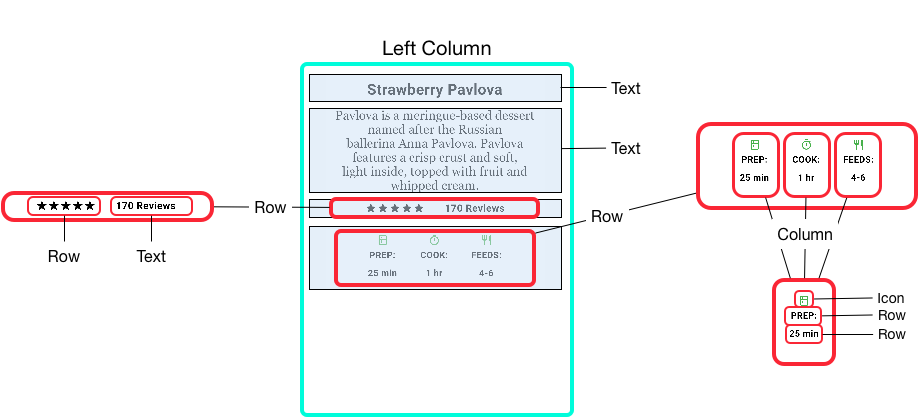
\includegraphics[width=0.9\linewidth]{img/flutter/layout_compose_detail.png}
    \caption{Compose widgets to create layout -- left column detailed~\cite{flutter-widget-layout}}
    \label{fig:flutter-compose-widget-detail}
\end{figure}
% --- # --- # --- # --- # --- # --- # --- # --- # --- # --- # --- # --- # --- # --- # --- # --- # --- # --- #
\subsection{Stateless vs Stateful Widget}
In the introduction it was said that Flutter's approach of displaying current user interface is declarative -- ``here is the current state of the application, draw something on the screen accordingly''.  In Flutter, whenever application' state changes, the user interface is redrawn. There is no imperative changing of the~\gls{ui}, such as \verb|textWidget.text = 'new text'|. The~advantage of the~declarative approach is that there is only one code path for any state of the~\gls{ui}. Developers just describe how the screen should look for a given state, and that is it~\cite{flutter-declarative}. The \gls{ui} can be described as a formula where \gls{ui} is equal to function which takes a state and returns new \gls{ui}~(\Cref{fig:flutter-ui-formula}).

\begin{figure}[htp]
    \centering
    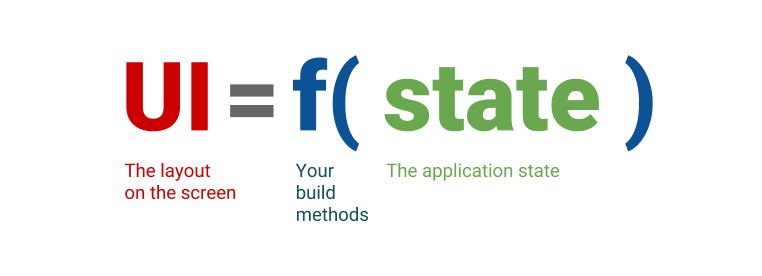
\includegraphics[width=0.6\linewidth]{img/flutter/ui_f_state.png}
    \caption{User interface formula~\cite{flutter-declarative}}
    \label{fig:flutter-ui-formula}
\end{figure}
% --- & --- & --- & --- & --- & --- & --- & --- & --- & --- & --- & --- & --- & --- & --- & --- & --- & --- &
\subsubsection{Build Context}
An~essential part of the widgets is \textit{BuildContext}. A~context is a~reference to the~location of the~widget within the~part of the~tree~\cite{notion-widget-didier}. Each widget has its own context. As~widgets are composed to the~tree, the contexts are as well. The widget has access to its own context and its parent context. 

The \textit{BuildContext} is provided to each widget through the~build method and is used to find the~widget's ancestors.  This is commonly used to obtain a~defined application theme or get a~reference to a~navigator widget, which is used to do navigation between screens. 
% --- & --- & --- & --- & --- & --- & --- & --- & --- & --- & --- & --- & --- & --- & --- & --- & --- & --- &
\subsubsection{Local vs. Application State}
The state is anything that forms what should be displayed. The state is any data what are needed in order to rebuild \gls{ui} at the~moment~\cite{flutter-local-app-state}. The~state can be separated into two concepts -- local state and application state. 

\begin{itemize}
    \item \textbf{Local state} -- Local state is which can be tied into one widget. It can be, for example, current tab in the ``tab selector'' widget, current progress of animation or state of checkbox (checked or unchecked).
    \item \textbf{Application state} -- Application State is which can not be local, whenever some information is needed to share across multiple widgets, the~state which should be kept during a~user session. An~example of application state can be a~logged user information, loaded articles from the~server or chat messages.
\end{itemize}
% --- & --- & --- & --- & --- & --- & --- & --- & --- & --- & --- & --- & --- & --- & --- & --- & --- & --- &
\subsubsection{Stateless Widget}
A~Stateless Widget is a widget which does not manage its own state. Once it gets its parameters, and it was built through the build method, it cannot be changed. Remember, that whenever Flutter decides to redraw the~screen, part of the~tree is rebuilt, but with new instances of the~widgets. Typical examples of the Stateless Widgets can be \textit{Container}, \textit{Text} or \textit{Icon}. These widgets accept many parameters which can alter their look (and behaviour), but they cannot be changed later on by~themselves. 
% --- & --- & --- & --- & --- & --- & --- & --- & --- & --- & --- & --- & --- & --- & --- & --- & --- & --- &
\subsubsection{Stateful Widget}
Whenever widget needs to manage its state and wants to mutate it for example, in case of an event, the widget should be stateful.  The widget as a~Stateless accepts parameters which can be used to configure this widget but also has an associated object, called state. This state object is an active part of the widget and is used to change widget and force framework rebuilt\gls{ui}. An~example of a \textit{Stateful Widget} can be a checkbox with ``checked'' state. 

Stateful Widget does not have only \verb|build()| method but has associated State object which defines several methods to support widget's lifecycle. These methods are \verb|initState()| for any state initialisation and \verb|dispose()| to clear any allocated resources. 

The state object is associated with widget's \textit{BuildContext}. This association is permanent, and state object will never change it~\cite{notion-widget-didier}. Even if the~Widget Context can be moved around the~tree structure, the~state will remain associated with that context. This implies that, the~Stateful Widget can be replaced during tree rebuild with new instance, but the~state object is persisted. 
% --- & --- & --- & --- & --- & --- & --- & --- & --- & --- & --- & --- & --- & --- & --- & --- & --- & --- &
\subsubsection{Force Rebuild with setState()}
As was mentioned, Stateful Widget can tell the framework to rebuild, and the widget can be redrawn based on the~changed state. The~Stateful Widget has method \verb|setState(callback)| which is used to do such rebuild. Inside \verb|callback| a developer should change the~widget's state to the~new value and framework will rebuild the widget based on that~new state. 
% --- & --- & --- & --- & --- & --- & --- & --- & --- & --- & --- & --- & --- & --- & --- & --- & --- & --- &
\subsubsection{Case Study: Counter Application}
Suppose application where are two buttons. One button increments a value (\verb|counter|) and other decrements. The counter value is displayed within two Text widgets located on different places within the application. Whenever any of the buttons are clicked, and the value is changed, all Text widgets should reflect this change.

\begin{figure}[htp]
    \centering
    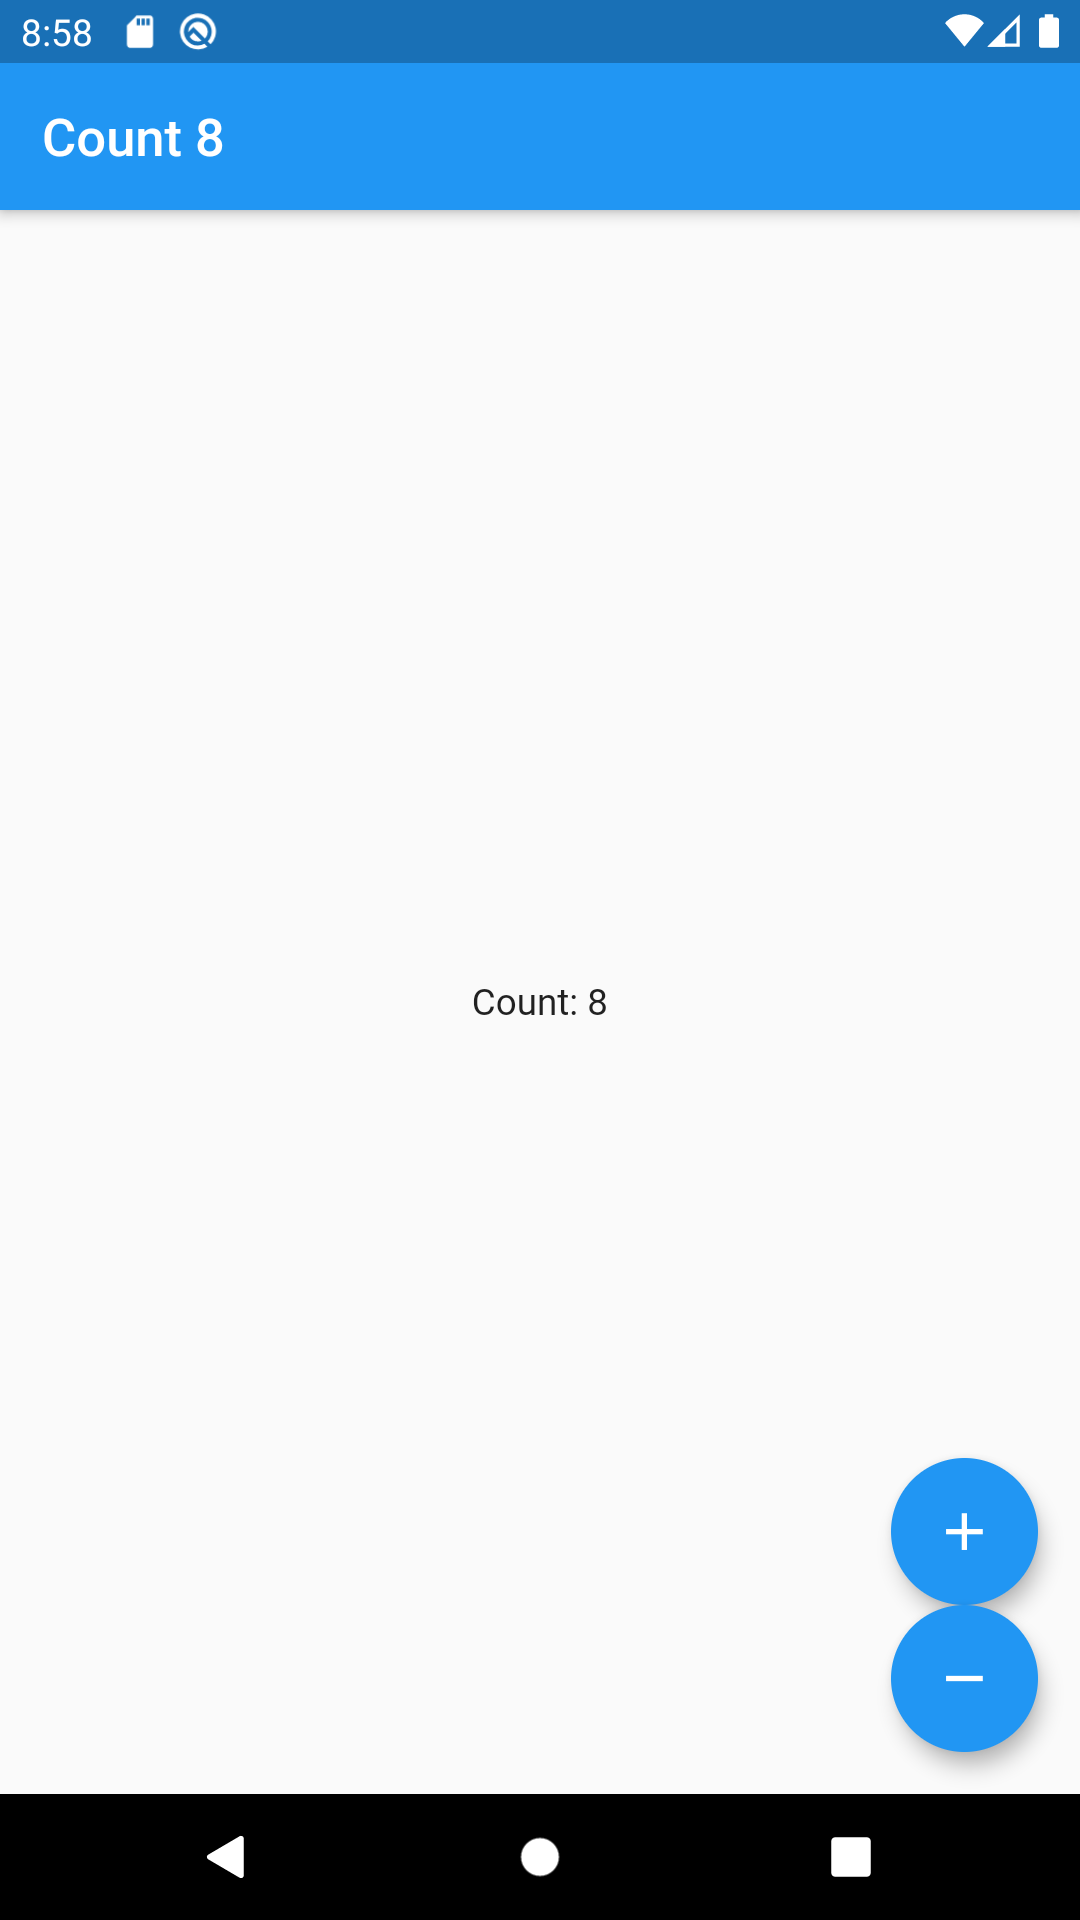
\includegraphics[width=0.33\linewidth]{img/flutter/counter_app_base.png}
    \caption{Counter application}
    \label{fig:counter-app}
\end{figure}

\begin{figure}[htp]
    \centering
    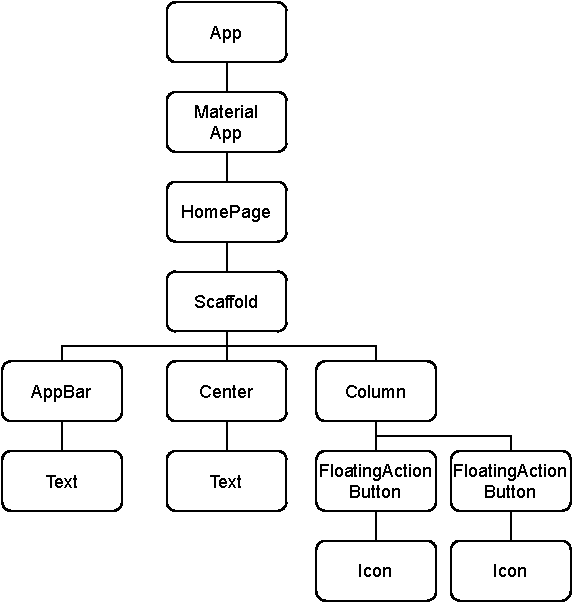
\includegraphics[width=0.75\linewidth]{img/flutter/counter-base.pdf}
    \caption{Counter application's widget tree}
    \label{fig:counter-app-widget-tree}
\end{figure}

Application's layout is shown in~\Cref{fig:counter-app} and the~corresponding widget tree in~\Cref{fig:counter-app-widget-tree} (shortened for brevity). In the \textit{AppBar} and in the centre of the screen, there is \textit{Text} widget which displays current value. On the bottom of the screen there are \textit{FloatingActionButtons} widgets, which increment (decrement) counter value. The value needs to be accessible to the Text and to the button as well. Hence, the state is declared within the whole application's widget \textit{HomePage}.  

\begin{listing}[ht]
\begin{minted}{dart}
class HomePage extends StatefulWidget {
  @override
  _HomePageState createState() => _HomePageState();
}
\end{minted}
\caption{HomePage widget definition}
\label{listing:counter-homepage-widget}
\end{listing}

\Cref{listing:counter-homepage-widget} shows the definition of the \textit{HomePage} widget. The widget inherits from \verb|StatefulWidget| and declares \textit{HomePageState} which is an associated state object.

\begin{listing}[ht]
\begin{minted}{dart}
class _HomePageState extends State<HomePage> {
  int _counter = 0;
  void _incrementCounter() => setState(() => _counter++);
  void _decrementCounter() => setState(() => _counter--);

  @override
  Widget build(BuildContext context) {
    return Scaffold(
      appBar: AppBar(title: CounterTextContainer(_counter)),
      body: Center(child: CounterTextContainer(_counter)),
      floatingActionButton: Column(
        children: <Widget>[
          FloatingActionButton(
            onPressed: _incrementCounter,
            child: Icon(Icons.add),
          ),
          FloatingActionButton(
            onPressed: _decrementCounter,
            child: Icon(Icons.remove),
          )]));
   }
}
\end{minted}
\caption{HomePageState -- setState example}
\label{listing:counter-base-state-homepage}
\end{listing}

\begin{listing}[ht]
\begin{minted}{dart}
class CounterTextContainer extends StatelessWidget {
  final int count;
  CounterTextContainer(this.count);
  
  @override
  Widget build(BuildContext context) {
    return Row(
        children: [
          const Icon(Icons.computer),
          const SizedBox(width: 5),
          Text('Count: $count')
        ],
    );
  }
}
\end{minted}
\caption{CounterTextContainer -- accepting state as parameter}
\label{listing:counter-base-text-container}
\end{listing}

\begin{figure}[htp]
    \centering
    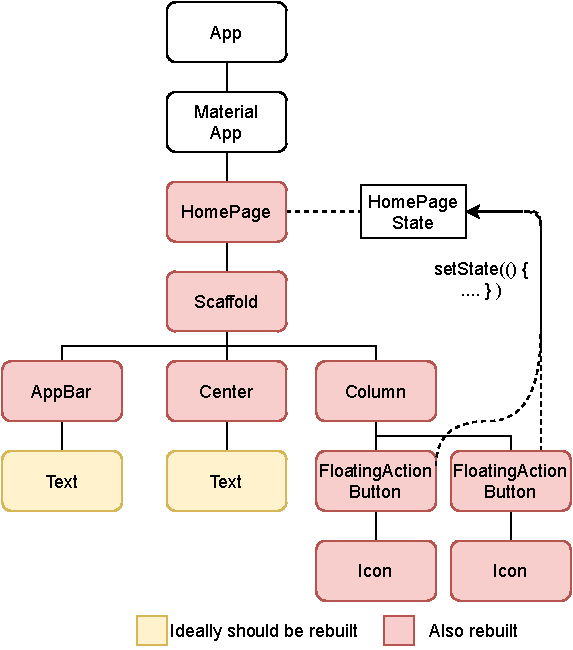
\includegraphics[width=0.75\linewidth]{img/flutter/counter-base-setState.pdf}
    \caption{Expected rebuilt vs actual rebuilt}
    \label{fig:counter-app-base-build}
\end{figure}

\Cref{listing:counter-base-state-homepage} shows definition of \textit{HomePageState} where state is represented as \verb|int _counter = 0| variable. There are also two private methods for incrementing and decrementing counter value. In each of the methods, the \verb|setState()| is called with the appropriate state change.  These two methods are bound to \verb|onPressed()| callback within \textit{FloatingActionButton}. The~state (\verb|_counter| variable) is passed down to~\verb|CounterTextContainer|~\Cref{listing:counter-base-text-container} where the value is used to display within \textit{Text} widget. 

The expectation is, that if the user pressed any of the buttons, the value is increment or decremented respectively and part of \gls{ui} which depends on \verb|_counter| value will be rebuilt. This part should be two Text widgets. In fact, the state is defined within the~\textit{HomePage} widget, and so, the~whole \textit{HomePage} and its children are rebuilt~(\Cref{fig:counter-app-base-build}). In~this small example, it is not really a~problem and performance should not be affected. However, if the~tree is deeply nested with heavy performance widgets (for example animations), it could lead to reduced performance and application can lags. 

How to define the application-wide state and prevent the necessary rebuilding part of the widget tree is a subject of ``state management'' section.
% ----- % ----- % ----- % ----- % ----- % ----- % ----- % ----- % ----- % ----- % ----- % ----- % ----- % ----- %
\section{State Management Approaches}
Using \verb|setState()| method is the~perfect solution (and recommended) for local state. However, as~soon as the state needs to be shared across multiple widgets, the managing this state becomes cumbersome. If the~state should be shared, there is only one viable solution -- \textbf{lifting state up}~\cite{flutter-simple-state-management}. The~state should reside in the widget, which is the parent for all widgets that needs access to the~state. Such a~solution can be used (and works) but creates a~few problems. 

The~very first problem is if some of the~interested widgets are kept in deep layers of the~tree and others are not, the~necessary amount of widgets is rebuilt whenever the state changes. The~second issue is that the~code of the widgets becomes very quickly hard to~manage due to its tight dependencies with upper widgets. The only doable solution to provide access to the~state is through references or function callbacks. These callbacks have to be passed to every widget down to the tree. This solution adds the~necessary complexity to maintenance and readability. Last but not least, the~application state usually has some business logic which should have been tested. However, if the~state (and its logic) is put directly into the widget, this logic is hard to test. 

The ``State Management'' is a~term for patterns and design solutions which helps to prevent those issues -- reducing necessary rebuilds, keeping code maintainable and testable. 
% --- # --- # --- # --- # --- # --- # --- # --- # --- # --- # --- # --- # --- # --- # --- # --- # --- # --- #
\subsection{Case Study Note}
In our case study, there are two places where the state (counter value) is needed -- first place is in the~AppBar's text and the centre of the screen. Secondly, the buttons for incrementing and decrementing need access to the~state in order to modify it. The first version of counter application used solution with \verb|setState()| and made the \textit{HomePage} (a root widget of the whole application) as \textit{StatefulWidget}. The~state was then accessible from every HomePage's children. Although this code is straightforward, there is already an~issue with the testability of the~business logic as it is tightly coupled to widget's class.  

Following lines in this section introduce some used patterns and solutions for state management.  Every solution will use the same case study but with appropriate implementation. Each solution's full code is available as an~appendix. The design and functionality remain the same as introduced before.
% --- # --- # --- # --- # --- # --- # --- # --- # --- # --- # --- # --- # --- # --- # --- # --- # --- # --- #
\subsection{Inherited Widget}
One solution offered by \textit{Flutter} framework is the concept of \textit{InheritedWidget}~\cite{flutter-inherited-widget}~\cite{notion-widget-didier}. This concept is used across the framework -- for example, obtaining current \textit{Theme} or screen device information through \textit{MediaQuery} object. Both can be accessed through convention ``of'' method -- \verb|Theme.of(context)| returns \textit{Theme} object. Internally these objects makes usage of InheritedWidget. InheritedWidget has two features:

\begin{itemize}
    \item It can be accessed from any widget directly.
    \item Whenever the widget changes, the accessing widget is automatically rebuilt.
\end{itemize}

The second implies that, for example, whenever widget access the~\textit{MediaQuery} and it is changed (the device is rotated, resolution changed,\ldots ), the widget is rebuilt to handle these changes. 

\begin{listing}[ht]
\begin{minted}{dart}
class _CounterInherited extends InheritedWidget {
  _CounterInherited({Widget child, this.data}) 
        : super(child: child);

  final CounterModel data;

  @override
  bool updateShouldNotify(_CounterInherited oldWidget) => true;
}
\end{minted}
\caption{\_CounterInherited}
\label{listing:counter-inherited-counter-inherited}
\end{listing}

\begin{listing}[ht]
\begin{minted}{dart}
class CounterModelProvider extends StatefulWidget {
  CounterModelProvider({this.child});
  
  final Widget child;
  
  @override
  CounterModel createState() => CounterModel();

  static CounterModel of(BuildContext context, 
                         {bool listen = true}) {
    return (listen
        ? context.
            dependOnInheritedWidgetOfExactType<_CounterInherited>()
        : context.
            findAncestorWidgetOfExactType<_CounterInherited>()
        )
        .data;
  }
}
\end{minted}
\caption{CounterModelProvider.}
\label{listing:counter-inherited-model-provider}
\end{listing}

\begin{listing}[ht]
\begin{minted}{dart}
class CounterModel extends State<CounterModelProvider> {
  int _count = 0;
  int get count => _count;

  void increment() => setState(() => _count++);
  void decrement() => setState(() => _count--);

  @override
  Widget build(BuildContext context) {
    return _CounterInherited(data: this, child: widget.child);
  }
}
\end{minted}
\caption{CounterModel}
\label{listing:counter-inherited-counter-model}
\end{listing}

\Cref{listing:counter-inherited-counter-inherited} is implementation of \textit{InheritedWidget}. It accepts child widget and \verb|CounterModel| which is state (and business logic) holding class (\Cref{listing:counter-inherited-counter-model}). The \verb|CounterModelProvider|~(\Cref{listing:counter-inherited-model-provider}) is a~widget which provides \verb|of(context, listen)| method and should be called when widget needs access to the model. The optional parameter \verb|listen| controls if a widget is automatically assigned to listening for changes or not. The \verb|of| method make usage of \verb|BuildContext| and traverses from given widget up to the~root until it finds the~widget searched for or fails. 

\begin{listing}[ht]
\begin{minted}{dart}
// MyApp - wraping HomePage with CounterModelProvider
home: CounterModelProvider(child: HomePage()),
// HomePage's build method
final model = CounterModelProvider.of(context, listen: false);
return Scaffold(
    appBar: AppBar(title: CounterTextContainer()),
    body: Center(child: CounterTextContainer()),
    floatingActionButton: Column(
      children: [
        FloatingActionButton(
          onPressed: model.increment,
          child: Icon(Icons.add),
        ),
        FloatingActionButton(
          onPressed: model.decrement,
          child: Icon(Icons.remove),
        )
      ],
));
\end{minted}
\caption{HomePage implementation (code simplified)}
\label{listing:counter-inherited-homepage}
\end{listing}

\begin{listing}[ht]
\begin{minted}{dart}
// CounterTextContainer's build method
return Row(
    children: [
      const Icon(Icons.computer),
      const SizedBox(width: 5),
      CounterText()
    ]);
//CounterText's build method
final model = CounterModelProvider.of(context);
return Text('Count: ${model.count}');
\end{minted}
\caption{CounterTextContainer and CounterText widgets}
\label{listing:counter-inherited-text-container}
\end{listing}

\begin{figure}[htp]
    \centering
    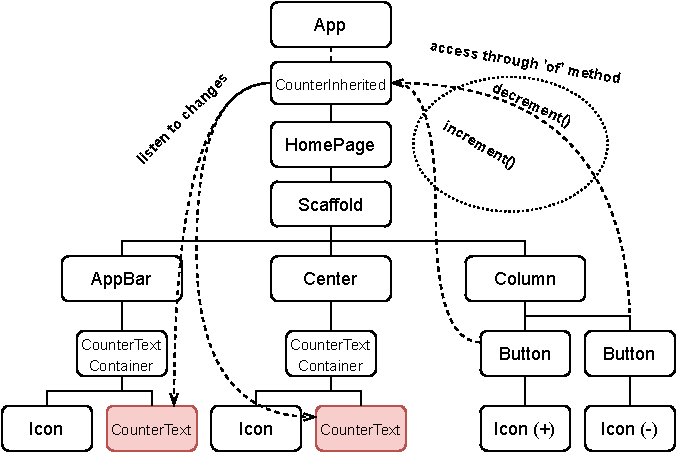
\includegraphics[width=0.75\linewidth]{img/flutter/counter-inherited-widget.pdf}
    \caption{InheritedWidget approach and its widget tree}
    \label{fig:counter-app-inherited-widget}
\end{figure}

The HomePage~(\Cref{listing:counter-inherited-homepage}) is wrapped by~\verb|CounterModelProvider| to provide access to any its children. Within the HomePage's \verb|build()| method, \verb|CounterModel| is obtained without listening. It is used for button's callbacks to invoke \verb|increment()| (\verb|decrement()| respectively) method. Inside \verb|CounterTextContainer| (\Cref{listing:counter-inherited-text-container}) is used Text widget and \verb|CounterText| where the~\verb|CounterModel| is accessed to get current value. Note that every widget is Stateless. The~most important thing is that only the~\textit{CounterText is rebuilt} when the~state changes~(see~\Cref{fig:counter-app-inherited-widget}) in comparison with \verb|setState| approach where the~whole application was rebuilt.

Although InheritedWidget solves many issues, the amount of code needed to achieve these results can be more unreadable and hard to maintain than approach with plain \verb|setState| method. However, Flutter's community created package which abstracts InheritedWidget and simplify this process. 
% --- # --- # --- # --- # --- # --- # --- # --- # --- # --- # --- # --- # --- # --- # --- # --- # --- # --- #
\subsection{Provider Package}

\begin{listing}[ht]
\begin{minted}{dart}
class CounterModel with ChangeNotifier {
  int _count = 0;
  int get count => _count;

  void increment() {
    _count++;
    notifyListeners();
  }

  void decrement() {
    _count--;
    notifyListeners();
  }
}
\end{minted}
\caption{Provider's CounterModel}
\label{listing:counter-provider-model}
\end{listing}

\begin{listing}[ht]
\begin{minted}{dart}
// in MyApp: provides CounterModel to descendants
home: ChangeNotifierProvider(
    create: (_) => CounterModel(),
    child: HomePage(),
),
// HomePage's build method
final model = Provider.of<CounterModel>(context, listen: false);
// ... rest of the HomePage's build method
// ... which is same as within InheritedWidget approach
\end{minted}
\caption{Provider's HomePage}
\label{listing:counter-provider-home-page}
\end{listing}

\begin{listing}[ht]
\begin{minted}{dart}
//CounterTextContainer build method
return Consumer<CounterModel>(
  builder: (context, model, child) {
    return Row(
        children: [
          child,
          const SizedBox(width: 5),
          Text('Count: ${model.count}') // CounterText
        ]);
  },
  // child widget is not rebuilt when model changes
  child: Container(
    padding: const EdgeInsets.all(8.0),
    child: Icon(Icons.computer),
  ),
);
\end{minted}
\caption{CounterTextContainer with Consumer}
\label{listing:counter-provider-consumer}
\end{listing}

\begin{figure}[ht]
    \centering
    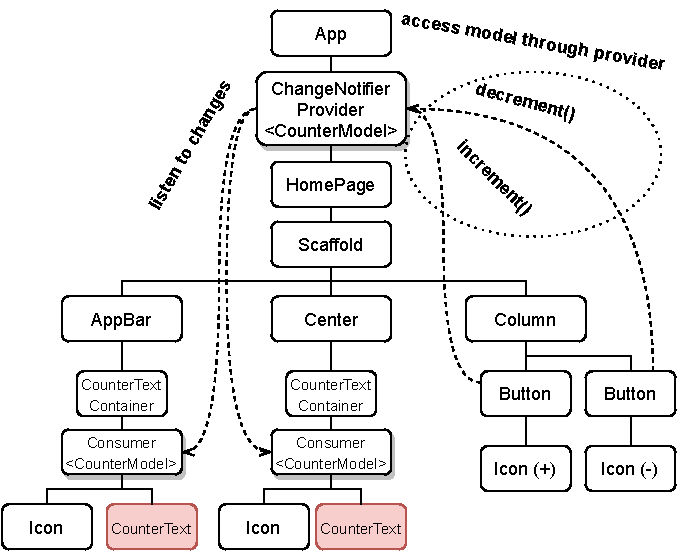
\includegraphics[width=0.75\linewidth]{img/flutter/counter-provider.pdf}
    \caption{Provider approach and its widget tree}
    \label{fig:counter-app-provider}
\end{figure}

Provider is a community package created by \textit{Remi~Rousselet}~\cite{package-provider} as a~simplification over inherited widgets with abstraction and more flexibility. One of the features is the concept of \verb|ChangeNotifier| and its \verb|ChangeNotifierProvider|. The concept behind is similar to the approach with the \verb|InheritedWidget|. The state is represented by the model class \verb|CounterModel|, which uses mixin \verb|ChangeNotifier|~(\Cref{listing:counter-provider-model}). This model contains only business logic and associated data. There are no widgets involved. If any of value is changed, the \verb|notifyListeners()| method should be called to notify its listeners to rebuilt.

The~\verb|ChangeNotifierProvider| wraps HomePage widget, where \verb|CounterModel| is created. Within HomePage's build method, the \verb|CounterModel| is accessed through \verb|Provider.of<CounterModel>(context, listen: false);| \\(note the~similarity with InheritedWidget) without listening to changes~(\Cref{listing:counter-provider-home-page}). The \verb|Consumer| widget used within \verb|CounterTextContainer|~(\Cref{listing:counter-provider-consumer}) allows to automatically listening to changes and re-run its \verb|builder| callback. If needed, the \verb|child| argument can be used to construct widget which can be part of the rebuilding widget without rebuilding itself. 

The result is the same as with \verb|InheritedWidget|~(\Cref{fig:counter-app-provider}), but with more readable code. The~\textit{Provider} package became very popular and encouraged by the Flutter team as a~solution for state management~\cite{flutter-simple-state-management}. Package offers more than the~\verb|ChangeNotifier| -- it can be used for dependency injection and it is used by many other packages such as~\textit{flutter\_bloc}~\cite{package-bloc}.
% --- # --- # --- # --- # --- # --- # --- # --- # --- # --- # --- # --- # --- # --- # --- # --- # --- # --- #
\subsection{Business Logic Component}
\gls{bloc} is a~pattern originally introduced by~\textit{Paolo Soares} and presented during \textit{DartConf~2018} conference~\cite{bloc-pattern-youtube}. The pattern was popularized by~\textit{Didier Boelens}~\cite{reactive-didier} and it was inspiration to \textit{Felix Angelov} for creation of~\textit{flutter\_bloc} package~\cite{package-bloc} -- a~popular BLoC based state management solution.

\begin{figure}[ht]
    \centering
    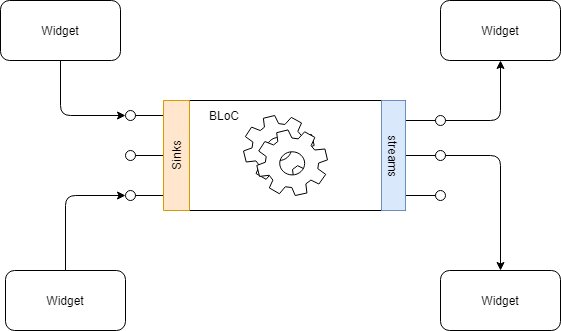
\includegraphics[width=0.6\linewidth]{img/flutter/bloc_pattern.png}
    \caption{A BLoC pattern~\cite{notion-widget-didier}}
    \label{fig:bloc-pattern}
\end{figure}

The \gls{bloc} builds on the streams. The \gls{bloc} stands for class, holding business logic where on one side accepts stream of events (event sink) and on the other side provides stream of states~(\Cref{fig:bloc-pattern}). Through event sinks, \gls{bloc} accepts events which are processed and based on them a new state is put to the state stream. In terms of Flutter -- widgets send events and listens for new state coming from state stream. The business logic itself is hidden from them and widgets (the~\gls{ui}) are concerned only about sending event and rebuilding themselves based on coming state.

The~\gls{bloc} solves the responsibility separation where the logic is centralised within the~\gls{bloc} class. This leads to better and easier testability. And~third, thanks to the~independence of \gls{ui} with business logic, changing and organizing layouts can be done without changes within the application's logic. The~\gls{ui} is only concerned about building widgets based on the current state and eventually sending events if needed. This also imply that events can be sent from any place within the application without any complexity.

\begin{figure}[ht]
    \centering
    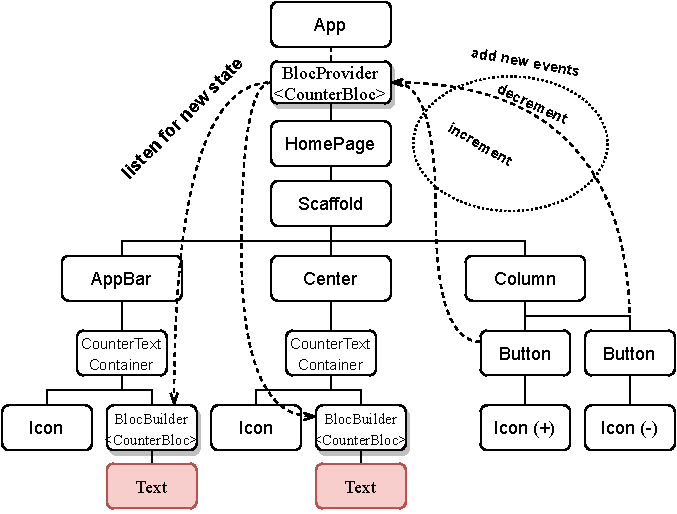
\includegraphics[width=0.75\linewidth]{img/flutter/counter-bloc.pdf}
    \caption{BLoC approach and its widget tree}
    \label{fig:counter-app-bloc}
\end{figure}

The \gls{bloc} also force centralized place where the particular state can be changed. With other solutions such as \textit{setState} and eventual callback passing, these changes can be spread across many places and it can be hard to maintain and test them. On the~other hand, the~usage of streams adds code complexity and robustness -- a~code boilerplate and the~application has to be designed with asynchronous execution in mind as the~\gls{bloc} relies on the~streams. The mentioned package \textit{flutter\_bloc} is \gls{bloc} pattern with abstraction over the stream's complexity without downgrading their usefulness and advantages. 

\subsubsection{flutter\_bloc Package}
\begin{listing}[ht]
\begin{minted}{dart}
// CounterBloc's events
enum CounterEvent { increment, decrement }

class CounterBloc extends Bloc<CounterEvent, int> {
  @override int get initialState => 0;

  @override
  Stream<int> mapEventToState(
    CounterEvent event,
  ) async* {
    if (event == CounterEvent.increment)
      yield state + 1;
    else if (event == CounterEvent.decrement) yield state - 1;
  }
}
\end{minted}
\caption{CounterBloc's implementation}
\label{listing:counter-bloc-bloc}
\end{listing}

\begin{listing}[ht]
\begin{minted}{dart}
// App' build method -- providing CounterBloc
home: BlocProvider(
        create: (_) => CounterBloc(),
        child: HomePage()),
        
// inside onPressed() callback - add event to bloc
context.bloc<CounterBloc>().add(CounterEvent.increment),
\end{minted}
\caption{BLoC approach -- providing CounterBloc and accessing bloc example}
\label{listing:counter-bloc-homepage}
\end{listing}

As before, the case study ``counter application'' was also written with the~\gls{bloc} approach. Widget tree and its rebuild~(\Cref{fig:counter-app-bloc}) is practically identical as with Provider. The difference lies in the how the code is organised, how the state is managed and the whole philosophy of the application's code. With \verb|InheritedWidget| the~state was mutated and its listeners were notified. With \gls{bloc} approach, whenever arrives new state, new state is returned and its listeners are rebuilt. 

\begin{listing}[ht]
\begin{minted}{dart}
Row(
children: <Widget>[
  const Icon(Icons.computer),
  const SizedBox(width: 5),
  BlocBuilder<CounterBloc, int>(
    builder: (context, state) => Text('Count: $state'),
  )]);
\end{minted}
\caption{BLoC approach -- CounterTextContainer's implementation}
\label{listing:counter-bloc-counter-text}
\end{listing}

The~\verb|flutter_bloc| has base \verb|Bloc<E,S>| class where \verb|E| is an ``event type'' and \verb|S| is a ``state type''. Each \gls{bloc} class has to inherit this base class and overrides ``mapEventToState'' method in order to respond to any event and \textit{yield} new state. How the~package works and how it can be used is more discussed in~\Cref{ch:implementation}. \Cref{listing:counter-bloc-bloc} shows \verb|CounterBloc| implementation. Events are represented as enum \verb|CounterEvent| with \textit{increment} and \textit{decrement} respectively. The state is simple \textit{integer} type. The \verb|flutter_bloc| package uses under the~hood \textit{Provider} so it is very similar how the~\gls{bloc} is provided to the widget tree. The bloc is accessed with \verb|context.bloc| in order to add new events. An example is shown at~\Cref{listing:counter-bloc-homepage}.  \verb|CounterTextContainer| widget (\Cref{listing:counter-bloc-counter-text}) uses \verb|BlocBuilder| widget which rebuilds whenever new state arrives. 
% --- # --- # --- # --- # --- # --- # --- # --- # --- # --- # --- # --- # --- # --- # --- # --- # --- # --- #
\subsection{Conclusion}
In this section, four approaches for state management was introduced. From simple \verb|setState| approach to stream based \gls{bloc}. As the \gls{bloc} encapsulates business logic into its own class and makes use of stream notion, this approach was chosen as the state management approach for implementation of our application due to convenient and straightforward way to usage, along with easy testability.
% ----- % ----- % ----- % ----- % ----- % ----- % ----- % ----- % ----- % ----- % ----- % ----- % ----- % ----- %
% \section{Native Features}
% \todo{How flutter can use native functions, e.g camera. Flutter plugins.}
% ----- % ----- % ----- % ----- % ----- % ----- % ----- % ----- % ----- % ----- % ----- % ----- % ----- % ----- %
\section{Flutter Internals}
In the last section of this chapter, some of the~internal Flutter's work is discussed. First of all, it is described more in-depth on how the framework is able to build widgets and draw them on the screen. Then the notion of Keys is introduced (an unique identification of widgets within widget tree). After that some optimisations such as const constructors which can give better performance are discussed. 

At the beginning of this chapter, \Cref{fig:flutter-layer-cake} shows how the Flutter is made. The middle layer - the engine is responsible for rendering and orchestrating Flutter framework. 
% --- # --- # --- # --- # --- # --- # --- # --- # --- # --- # --- # --- # --- # --- # --- # --- # --- # --- #
\subsection{RenderObject and RenderTree}
As was said earlier, Flutter uses pixel-perfect rendering -- each Widget is in the end translated into several pixels drawn on the screen. In order to do that, engine has a notion of the Render Tree.

The RenderTree is composed by objects called RenderObjects. These RenderObjects are used to define~\cite{didier-internals}:
\begin{itemize}
    \item define some area of the screen in terms of dimensions, position, geometry but also in terms of ``rendered content'',
    \item identify zones of the screen potentially impacted by the gestures,
\end{itemize}
The root object of the tree is called RenderView.
% --- # --- # --- # --- # --- # --- # --- # --- # --- # --- # --- # --- # --- # --- # --- # --- # --- # --- #
\subsection{Everything is a Widget Revisited}
From a developer perspective, everything is a widget what is related to the~\gls{ui} in terms of layout and interaction~\cite{didier-internals}. The~Widget is an immutable class, where instances (or more precise its derivates) form the widget tree by composition. The~Widget itself, however, does not know how it can be rendered to the~screen. 

\begin{figure}[ht]
    \centering
    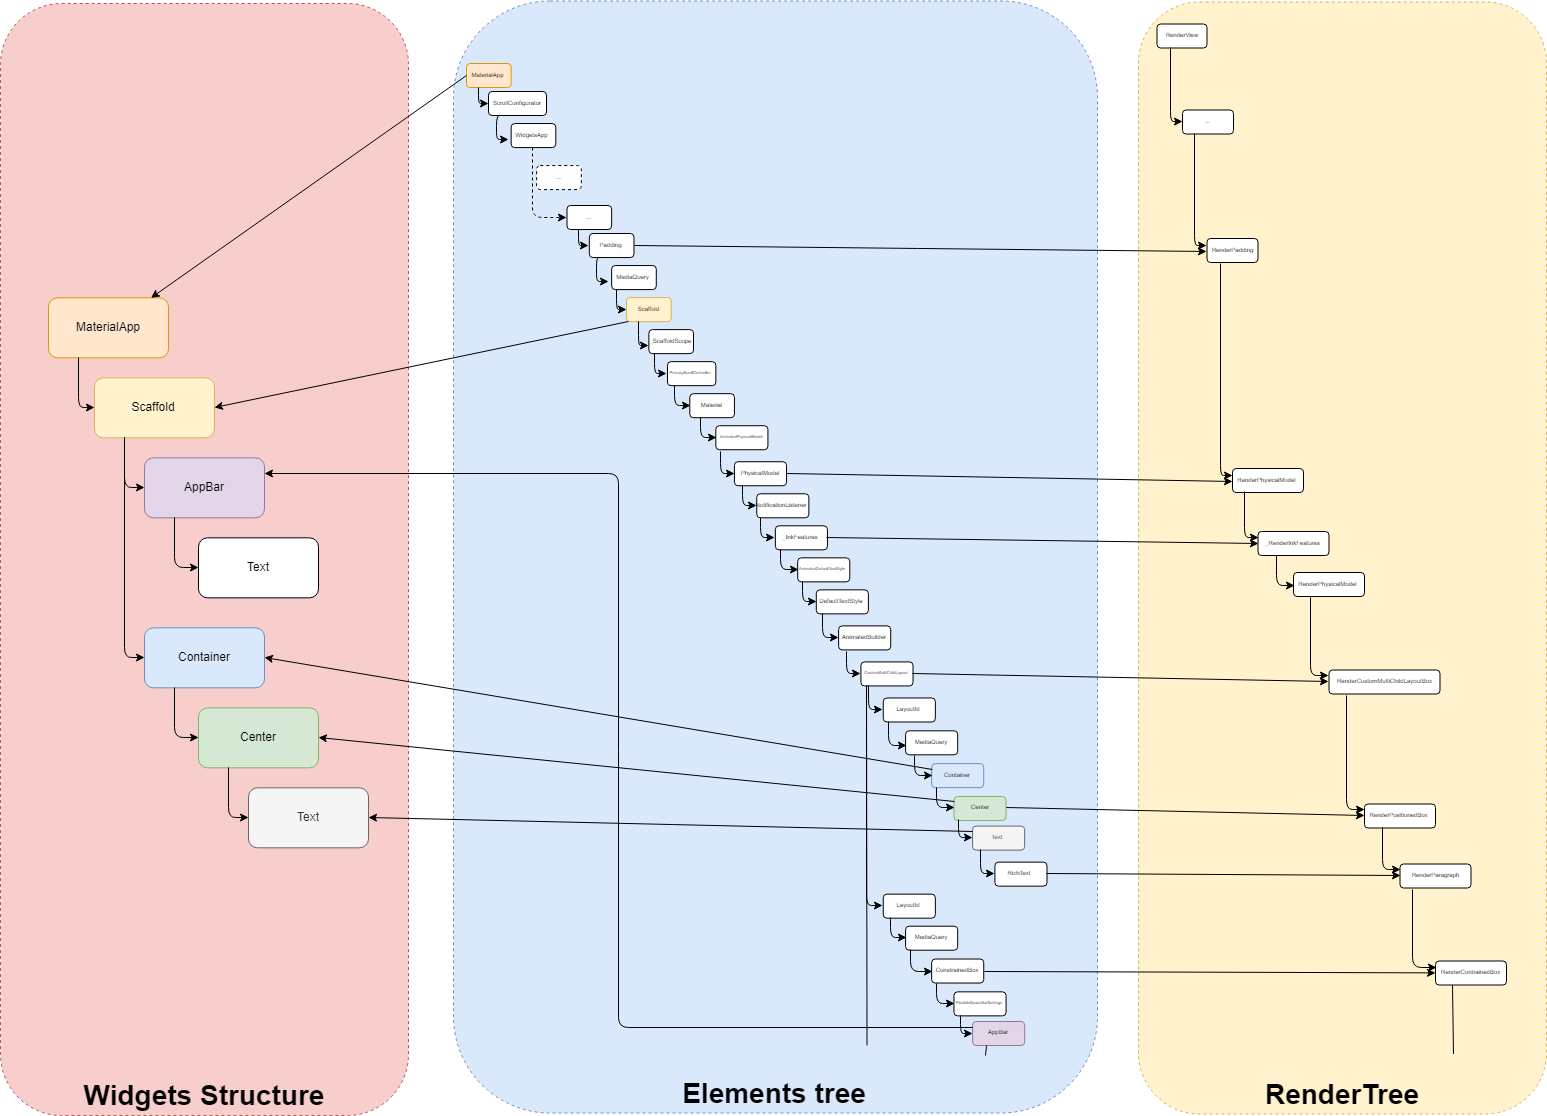
\includegraphics[width=0.75\linewidth]{img/flutter/internals_3_trees.png}
    \caption{Three trees -- Widget, Element and Render Tree~\cite{didier-internals}.}
    \label{fig:flutter-internal-3-trees}
\end{figure}

When Flutter needs to render the current state to the screen, the engine will request to inflate all widgets~\cite{didier-internals}. This can be simplified as unpacking the ``box of boxes''. Each Widget internally uses more granulated, and low-level API's Widgets in order to precisely describe the layout. Furthermore, from a developers perspective, the widgets create Widget tree. In fact, internally each Widget has assigned \textit{Element} object which forms the \textit{Element Tree}.

Each Element points to Widget which created it, parent and potentially child Element and may also point to a RenderObject~\cite{didier-internals}.  \Cref{fig:flutter-internal-3-trees} shows notion of ``widget tree'', Element~Tree and Render~Tree.

Every Widget can be assigned to one of the three categories~\cite{didier-internals}:
\begin{enumerate}
\item \textbf{The proxies}  -- these Widgets hold information which needs to be available to other Widgets -- such as \verb|InheritedWidget|.
\item \textbf{The Renderer}s -- These Widgets define the layout of the screen, such as Row, Column, Padding, \ldots
\item \textbf{The Components} -- These Widgets provide final information related to how the piece of~\gls{ui} should look. An~example of such a Widget can be Text or RaisedButton. 
\end{enumerate}
Depending on the Widget category, a corresponding Element type is associated. There are two main Element types - \textit{ComponentElement} and \textit{RenderObjectElement}. The first one does not directly correspond to visual rendering. The latter one has a connection to RenderObjects.  Also, every Widget has its corresponding Element object, speaking of StatefulWidget has corresponding StatefulElement where the state is associated. This statement also implies that BuildContext is Element itself. 
% --- # --- # --- # --- # --- # --- # --- # --- # --- # --- # --- # --- # --- # --- # --- # --- # --- # --- #
\subsection{Deciding What to Redraw}
A redraw mechanic relies on invalidating either an Element or a RenderObject~\cite{didier-internals}.  Whenever the Widget should be rebuilt, the corresponding Element is marked as dirty. Invalidation of RenderObject can happen, for example, when changes to its dimension, position or geometry are made or when the Element tree is marked as dirty. When engine decides that new repaint should happen, it iterates over all invalidated (dirty) elements and request them to rebuild. Internally the rebuild works as~\cite{didier-internals}:
\begin{quote}
    \begin{enumerate}
    \item The corresponding Widget's build method is called which returns a new Widget.
    \item If the Element has no child, the~new Widget is inflated.
    \item Otherwise the new Widget is compared to the one referenced by the~child element and
        \begin{itemize}
        \item if they are same (same widget type and Key), the update is made and the child element in the~Element Tree is kept,
        \item if they are not same, the child element is unmounted (and discarded) and the new Widget is inflated.
        \end{itemize}
    \item The inflating of the Widget leads to creating a new element, which is inserted into the element tree as a new child of the Element. 
    \end{enumerate}
\end{quote}


After that, the ElementTree is considered as a stable and a similar process is made with Render Tree -- every RenderObject marked as dirty performs its layout (calculating dimension and geometry), every RenderObject marked to repaint is repainted. In the end, the device screen is redrawn. 
% --- # --- # --- # --- # --- # --- # --- # --- # --- # --- # --- # --- # --- # --- # --- # --- # --- # --- #
\subsection{Notion of Keys}
When comparing new Widget with current one within Element, the Element decides to rebuild when the Widget type and Key are different. A \textit{Key} is an object associated with a Widget. In the simplest form, a Key can be considered as the unique identification of the Widget. In most cases, developers should not need to work with the keys as Flutter manage them internally. However, there are cases where the manual definition of the Key is necessary. 

\begin{figure}[ht]
    \centering
    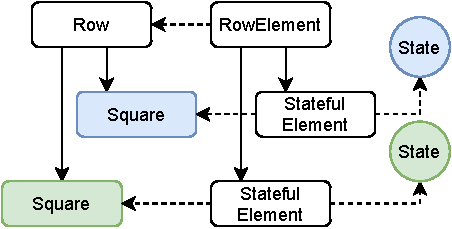
\includegraphics[width=0.75\linewidth]{img/flutter/key_stateful_start.pdf}
    \caption{Square Widgets and associated Elements with States}
    \label{fig:keys_start}
\end{figure}

\begin{figure}[ht]
    \centering
    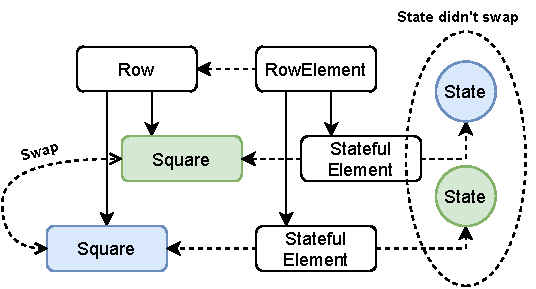
\includegraphics[width=0.75\linewidth]{img/flutter/key_stateful_wrong_state.pdf}
    \caption{Square Widgets after swap and associated Elements with wrong States}
    \label{fig:keys_wrong}
\end{figure}

\begin{listing}[ht]
\begin{minted}{dart}
// SquarePage holds list of Square widgets
class _SquaresPageState extends State<SquaresPage> {
  final squares = [Square(RandomColor.get()), 
                    Square(RandomColor.get())];
  void _shiftSquares() {
    setState(() => squares.insert(1, squares.removeAt(0)));
  }

  @override
  Widget build(BuildContext context) {
    return Scaffold(
        body: Row(children: squares),
        floatingActionButton: FloatingActionButton(
          onPressed: _shiftSquares,
          //...
        ),
      );
   }
}
\end{minted}
\caption{SquarePage widget with Stateless Square widgets}
\label{listing:keys_page_stateless}
\end{listing}

The problem can occur when some Widget uses a collection of Widgets of the~same type that holds some state.  Consider a concrete example where \verb|SquarePage| holds a list of \verb|Square| widgets~(\Cref{listing:keys_page_stateless}). Each \verb|Square| (as a StatelessWidget) has defined random colour through a constructor. After a~button is clicked, the squares are swapped. With \verb|Square| as StatelessWidgets, everything works as expected. 

\begin{listing}[ht]
\begin{minted}{dart}
class Square extends StatefulWidget {
  Square({Key key}) : super(key: key);
  @override
  _SquareState createState() => _SquareState();
}

class _SquareState extends State<Square> {
  Color color;
  @override
  void initState() {
    color = RandomColor.get();
  }

  @override
  Widget build(BuildContext context) {
    return Container(color: color,width: 100,height: 100);
  }
}
\end{minted}
\caption{Square widget as StatefulWidget}
\label{listing:keys_square_stateful}
\end{listing}

However, if the~\verb|Square| becomes StatefulWidget~(\Cref{listing:keys_square_stateful}) and the button is clicked, it seems like nothing happened -- squares stay on the same place. As was said when the~Widget is marked to rebuilt, it walks through Elements and if the Widget type and the Key match the Element updates its reference to new Widget. In the~case of StatefulWidget, the associated state is linked to the~Element object~(\Cref{fig:keys_start}). When squares are shifted, the~Element is marked as dirty. It walks through square's StatefulElement and checks if Widget type and Key matches -- and they are as no Keys are assigned. Hence, the~Element updates its Widget reference, but the~associated state remains the~same~(\Cref{fig:keys_wrong}). 
The key is to add Key. There are several types of Keys such as ValueKey, where some unique value can be assigned (for example article's id). For \verb|Square| example, the \textit{UniqueKey} which generates unique identification is enough.  After the Keys are assigned, \mint{dart}|final squares = [Square(key: UniqueKey()),Square(key: UniqueKey())]| the example works again as expected. The~full example code is available as~before within appendix.

The keys should be put to the most top Widget, which is used as a root widget of collection. Otherwise, the rebuilding algorithm fails once again, and wrong behaviour will occur. In practice, Key should be used when stateful widgets are used within collections (such as ListView, Row or Column) and they are manipulated -- moved, removed and similar.  Moreover, sometimes the GlobalKey can be used to manage some Widget's state ``outside''. This approach is often used with managing text inputs. 
% --- # --- # --- # --- # --- # --- # --- # --- # --- # --- # --- # --- # --- # --- # --- # --- # --- # --- #
\subsection{Const Optimisation}
On of the Dart's features are \textit{const} constructors which makes instance as a~\textit{compile-time constant}. This feature can be used to optimise widget builds and prevent unnecessary rebuilds. Most of the Widgets has \textit{const} constructor, and if possible, the~\textit{const} constructor should be used. Such as Icon widget or Text widget if they accept non-changing values they can be made compile-time constants and Flutter when rebuilding the tree will these Widget reuses instead of creating a new one. 

The problem of performance optimisation is a vast subject for discussion, and it could have its own chapter. The~const constructors are only ``tip of the iceberg''. In general, it is somewhat common sense to~avoid unnecessary \gls{ui} rebuilds or avoid using animations carelessly such as animate each line of Text within ListView whenever the~list is updated. Some other optimisation tips are discussed later in the~implementation chapter. 

\section{Conclusion}
The first chapter introduced Flutter framework and its philosophy ``everything is a widget'' as a~primary user interface building block. The~notion of state and several state management approaches were discussed, how they can be implemented and how they affect the rebuilding of~\gls{ui}. In the~end, part of Flutter internals was uncovered and explained to grasp a better understanding of how the~framework works.